%% FEUP THESIS STYLE for LaTeX2e
%% how to use feupteses (English version)
%%
%% FEUP, JCL & JCF, 31 July 2012
%%
%% PLEASE send improvements to jlopes at fe.up.pt and to jcf at fe.up.pt
%%

%%========================================
%% Commands: pdflatex tese
%%           bibtex tese
%%           makeindex tese (only if creating an index)
%%           pdflatex tese
%% Alternative:
%%          latexmk -pdf tese.tex
%%========================================

\documentclass[11pt,a4paper,twoside,openright]{report}

%% For iso-8859-1 (latin1), comment next line and uncomment the second line
\usepackage[utf8]{inputenc}
\usepackage{subcaption}
\usepackage{amsmath}
%\usepackage[latin1]{inputenc}

%% English version

%% MIEIC options
%\usepackage[mieic]{feupteses}
%\usepackage[mieic,juri]{feupteses}
%\usepackage[mieic,final]{feupteses}
%\usepackage[mieic,final,onpaper]{feupteses}

%% MIEEC options
%\usepackage[mieec]{feupteses}
%\usepackage[mieec,juri]{feupteses}
%\usepackage[mieec,final]{feupteses}

%% For other degrees
\usepackage{feupteses} % you must define the degree bellow

%% Additional options for feupteses.sty: 
%% - onpaper: links are not shown (for paper versions)
%% - backrefs: include back references from bibliography to citation place

%% Uncomment to create an index (at the end of the document)
%\makeindex
\graphicspath{{figures/}}

%%----------------------------------------
%% TIP: if you want to define more macros, use an external file to keep them
%some macro definitions

% format
\newcommand{\class}[1]{{\normalfont\slshape #1\/}}

% entities
\newcommand{\Feup}{Faculdade de Engenharia da Universidade do Porto}

\newcommand{\mc}[1]{\mathcal{#1}}
\newcommand{\mb}[1]{\mathbf{#1}}

%%----------------------------------------

%%========================================
%% Start of document
%%========================================
\begin{document}

%%----------------------------------------
%% Information about the work
%%----------------------------------------
\title{Dissertation Preparation}
\author{José Pedro Castro Fonseca}

%% Comment next line if not necessary for degree
\degree{Integrated Masters in Electrical and Copmuter Engineering}

%% Uncomment next line for date of submission
%\thesisdate{July 31, 2008}

%% Comment next line copyright text if not used
\copyrightnotice{José Fonseca, 2016}

\supervisor{Supervisor}{João Canas Ferreira}
\supervisor{Second Supervisor}{Ivo Timóteo}

%% Uncomment next line if necessary
%\supervisor{Second Supervisor}{Name of the Supervisor}

%% Uncomment committee stuff in the final version if used
%\committeetext{Approved by \ldots:}
%\committeemember{President}{Name of the President}
%\committeemember{Referee}{Name of the Referee}
%\committeemember{Referee}{Name of the Referee}
%\signature

%% Specify cover logo (in folder ``figures'')
\logo{uporto-feup.pdf}

%% Uncomment next line for additional text below the author's name (front page)
%\additionalfronttext{Preparação da Dissertação}

%%----------------------------------------
%% Preliminary materials
%%----------------------------------------

% remove unnecessary \include{} commands
\begin{Prolog}
  \chapter*{Resumo}
%\addcontentsline{toc}{chapter}{Resumo}

Este documento ilustra o formato a usar em dissertações na \Feup.
São dados exemplos de margens, cabeçalhos, títulos, paginação, estilos
de índices, etc. 
São ainda dados exemplos de formatação de citações, figuras e tabelas,
equações, referências cruzadas, lista de referências e índices.
Este documento não pretende exemplificar conteúdos a usar. 
É usado o \emph{Loren Ipsum} para preencher a dissertação.

Lorem ipsum dolor sit amet, consectetuer adipiscing elit. Etiam vitae
quam sed mauris auctor porttitor. Mauris porta sem vitae arcu sagittis
facilisis. Proin sodales risus sit amet arcu. Quisque eu pede eu elit
pulvinar porttitor. Maecenas dignissim tincidunt dui. Pellentesque
habitant morbi tristique senectus et netus et malesuada fames ac
turpis egestas. Donec non augue sit amet nulla gravida
rutrum. Vestibulum ante ipsum primis in faucibus orci luctus et
ultrices posuere cubilia Curae; Nunc at nunc. Etiam egestas. 

Donec malesuada pede eget nunc. Fusce porttitor felis eget mi mattis
vestibulum. Pellentesque faucibus. Cras adipiscing dolor quis
mi. Quisque sagittis, justo sed dapibus pharetra, lectus velit
tincidunt eros, ac fermentum nulla velit vel sapien. Vestibulum sem
mauris, hendrerit non, feugiat ac, varius ornare, lectus. Praesent
urna tellus, euismod in, hendrerit sit amet, pretium vitae,
nisi. Proin nisl sem, ultrices eget, faucibus a, feugiat non,
purus. Etiam mi tortor, convallis quis, pharetra ut, consectetuer eu,
orci. Vivamus aliquet. Aenean mollis fringilla erat. Vivamus mollis,
purus at pellentesque faucibus, sapien lorem eleifend quam, mollis
luctus mi purus in dui. Maecenas volutpat mauris eu lectus. Morbi vel
risus et dolor bibendum malesuada. Donec feugiat tristique erat. Nam
porta auctor mi. Nulla purus. Nam aliquam. 


\chapter*{Abstract}
%\addcontentsline{toc}{chapter}{Abstract}

Here goes the abstract written in English.

Lorem ipsum dolor sit amet, consectetuer adipiscing elit. Sed vehicula
lorem commodo dui. Fusce mollis feugiat elit. Cum sociis natoque
penatibus et magnis dis parturient montes, nascetur ridiculus
mus. Donec eu quam. Aenean consectetuer odio quis nisi. Fusce molestie
metus sed neque. Praesent nulla. Donec quis urna. Pellentesque
hendrerit vulputate nunc. Donec id eros et leo ullamcorper
placerat. Curabitur aliquam tellus et diam. 

Ut tortor. Morbi eget elit. Maecenas nec risus. Sed ultricies. Sed
scelerisque libero faucibus sem. Nullam molestie leo quis
tellus. Donec ipsum. Nulla lobortis purus pharetra turpis. Nulla
laoreet, arcu nec hendrerit vulputate, tortor elit eleifend turpis, et
aliquam leo metus in dolor. Praesent sed nulla. Mauris ac augue. Cras
ac orci. Etiam sed urna eget nulla sodales venenatis. Donec faucibus
ante eget dui. Nam magna. Suspendisse sollicitudin est et mi. 

Fusce sed ipsum vel velit imperdiet dictum. Sed nisi purus, dapibus
ut, iaculis ac, placerat id, purus. Integer aliquet elementum
libero. Phasellus facilisis leo eget elit. Nullam nisi magna, ornare
at, aliquet et, porta id, odio. Sed volutpat tellus consectetuer
ligula. Phasellus turpis augue, malesuada et, placerat fringilla,
ornare nec, eros. Class aptent taciti sociosqu ad litora torquent per
conubia nostra, per inceptos himenaeos. Vivamus ornare quam nec sem
mattis vulputate. Nullam porta, diam nec porta mollis, orci leo
condimentum sapien, quis venenatis mi dolor a metus. Nullam
mollis. Aenean metus massa, pellentesque sit amet, sagittis eget,
tincidunt in, arcu. Vestibulum porta laoreet tortor. Nullam mollis
elit nec justo. In nulla ligula, pellentesque sit amet, consequat sed,
faucibus id, velit. Fusce purus. Quisque sagittis urna at quam. Ut eu
lacus. Maecenas tortor nibh, ultricies nec, vestibulum varius, egestas
id, sapien. 

Donec hendrerit. Vivamus suscipit egestas nibh. In ornare leo ut
massa. Donec nisi nisl, dignissim quis, faucibus a, bibendum ac,
diam. Nam adipiscing hendrerit mi. Morbi ac nulla. Nullam id est ac
nisi consectetuer commodo. Pellentesque aliquam massa sit amet
tellus. Vivamus sodales aliquam leo. 
 % the abstract
  \chapter*{Agradecimentos}
\addcontentsline{toc}{chapter}{Acknowledgements}

Agradeço a todos os professores que se cruzaram comigo na minha vida e que, através da sua ação,
me transmitiram os conhecimentos necessários para me formar como Engenheiro e produzir este trabalho,
que espero que seja de uso para a comunidade científica e para a Humanidade. Uma palavra especial
ao meu orientador deste trabalho, o Prof. João Canas Ferreira, que desde o primeiro momento acolheu
esta proposta de trabalho e soube ver nela o seu potencial devido, e ao co-orientador, o Ivo Timóteo,
que mais do que minha referência para a parte teórica deste trabalho, é um bom amigo.

Agradeço todo o esforço da comunidade \textit{open-source} que desenvolveu grande parte das ferramentas
com que trabalhei, desde o \LaTeX~ em que escrevi este documento, ao \href{https://www.python.org/}{Python} e \href{http://www.numpy.org/}{Numpy}
usado na automatização de tarefas e no teste duma primeira versão software da rede. Agradeço também ao autor das \href{https://ece.uwaterloo.ca/~aplevich/Circuit_macros/}{Circuit Macros},
J.D. Aplevich, que muito foram úteis para a elaboração de quase todos os diagramas deste trabalho.

Uma última palavra de apreço para as pessoas especiais da minha vida. Os meus pais, que me formaram como Pessoa e me
incutiram força em todos os momentos da vida, do qual esta tese não é excepção, e à minha namorada, a Mafalda, que apesar
de não ser da minha área, sempre se entusiasmou e interessou por todos os progressos que fui atingindo ao longo destes meses.

\vspace{10mm}
\flushleft{José Pedro Castro Fonseca}
  % the acknowledgments
  \cleardoublepage
\thispagestyle{plain}

\vspace*{8cm}

\begin{flushright}
   \textsl{``You should be glad that bridge fell down. \\
           I was planning to build thirteen more to that same design''} \\
\vspace*{1.5cm}
           Isambard Kingdom Brunel
\end{flushright}
    % initial quotation if desired
  \cleardoublepage
  \pdfbookmark[0]{Table of Contents}{contents}
  \tableofcontents
  \cleardoublepage
  \pdfbookmark[0]{List of Figures}{figures}
  \listoffigures
  \cleardoublepage
  \pdfbookmark[0]{List of Tables}{tables}
  \listoftables
  \chapter*{Abbreviations and Symbols}
%\addcontentsline{toc}{chapter}{Abbreviations}
\chaptermark{Abbreviations and Symbols}

\begin{flushleft}
\begin{tabular}{l p{0.8\linewidth}}
ANN      & Artificial Neural Networks\\
BPTT     & Backpropagation Through Time\\
CNN      & Convolutional Neural Network\\
CPU      & Central Processing Unit\\
FPGA     & Field-Programmable Gate Array\\
LSTM     & Long Short-Term Memory\\
RNN      & Recursive Neural Networks\\
SPSA     & Simultaneous Perturbation Stochastic Approximation\\
\end{tabular}
\end{flushleft}

  % the list of abbreviations used
\end{Prolog}

%%----------------------------------------
%% Body
%%----------------------------------------
\StartBody

%% TIP: use a separate file for each chapter
\chapter{Theoretical Background}\label{chap:theorBack}


\section{Basic Concepts of Machine Learning}
Machine Learning is a field of Computer Science that studies the development of mathematical techniques that allow software to learn autonomously, without an explicit description of each rule of operation. Its goal is to extract latent features from the data that allow an immediate classification of each input data into a particular class -- the catch is that there is no previous rule formulation, but instead we have an adaptive model that adjusts is parameters accordingly with the input data it receives, improving the estimates it yields as it receives new input samples. 

Let us consider a practical example. For instance, suppose we want to build a program that given an input audio waveform representation of a spoken word, it matches it into a particular word of a dictionary. We could, of course, devise a set of rules and exceptions for each word analysing some of its features (perhaps the Fourier representation of each one, and, from it, manually finding the appropriate rules for each), but apart from it being a very complex task, it wouldn't be a scalable solution, given the enormous number of words in each language. The approach taken by Machine Learning is diametrically different, and instead of manually processing each waveform, we build a large dataset, of size $N$, containing the waveforms of several words $\left[ \mb{x}_1 \; \mb{x}_2 \;\mb{x}_2 \; \dots \mb{x}_N \right]$ -- we call this dataset the \textbf{training dataset} -- and we feed it to our model. Each of the $i$-th data point was previously labelled, and in fact we feed each training data point $\mb{x}_i$ \emph{along} with its corresponding label $t_i$, so that the model can adapt its parameters accordingly to the \emph{target value} it is supposed to classify. This set of labels $\mb{t} = \left[ t_1 \; t_2 \; t_3 \; \dots \; t_N \right]$ is called the \textbf{target vector}. 

We are, then, left with the following question: how can the model quantitatively evaluate the quality of its current set of parameters? That could be achieved in a number of ways, but the most usual is using a \textbf{Cost Function} that, as the name suggests, measures the cost of each wrong classification of the model. The model then evolves in a way that minimizes the cost function. A usual choice for the cost function is the \textbf{sum of squares error}. Mathematically, if $y_{\theta}^i = y_{\theta}(x_i)$ is the prediction for the input data point $x_i$ with label $t_i$, given the current set of parameters $\theta$, the cost function using this metric is given by

\begin{equation}\label{eq:costfunctionFund}
	J(\theta) = \frac{1}{2} \sum_{i=1}^N \left( y_{\theta}^i - t_i \right)^2.
\end{equation}

Sometimes, instead of applying the raw data to the model, we can apply some sort of \emph{preprocessing} to the data to extract the relevant features from it. For instance, instead of just feeding a raw image, we can perform several operations like edge detection or low-pass filtering, and apply them in parallel. In cases of highly dimensional data (i.e. each data vector has a very high number of features), we can apply techniques like \textbf{Principal Component Analysis} to reduce the feature space to a smaller dimension one, where the previous features were combined into two or three new features that pose themselves as the most relevant.

The problems described above are, in fact, a subset of the problems that Machine Learning tries to address. These problems are called \textbf{classification problems}, because for each input data point, our model tries to fit it into the most appropriate class. But we can also address \textbf{regression problems} where the output is not limited to a discrete set of values but rather a continuous interval. On the other hand, the Neural Network that this work will implement addresses a special kind of classification problem, where the classification decision is influenced not only by the current input sample, but also by a given \emph{window of samples} that trail the current sample.

In summary, the most typical setting for a Machine Learning problem is having a large \textit{input dataset} which we use to \textit{train} our model (i.e. allowing him to dynamically adapt its set of parameters $\theta$), in order to produce an output label $y_i$ for each of them that minimizes a quality metric, the \textit{Cost Funcion}, which can be chosen to the sum of squared differences, the log-loss, or any other appropriate  mathematical relationship  between the estimate $y_i$ and the correct label $t_i$. 

Now that the basic Machine Learning concepts have been presented, I will discuss, henceforth, one of the most important algorithms that address the supervised classification problems, the \emph{Artificial Neural Networks} that will be discussed in Section~\ref{sec:theorBack_ann} as somewhat of a contextual introduction to the main theme of the thesis, which will be Recurrent Neural Networks (Section~\ref{sec:theorBack_rnn}), namely the \textbf{Long Short-Term Memory Networks} (Section~\ref{sec:theorBack_lstm}), both of which are improvements over the initial formulation of the ANNs. These two last networks branch even further from these set of problems, and are usually employed in \textit{Deep Learning} tasks, where we try to extract even higher level information from data at the expense of increased model complexity. 

\section{Artificial Neural Networks}\label{sec:theorBack_ann}

Artificial Neural Networks (ANN) are mathematical structures that, as the name suggests, try to mimic the Human Brain. ANN's building blocks, like their biological counterpart, model the high-level behaviour of biological neurons, in the sense that they neglect unnecessary biological aspects (such as modeling all the voltages across the neuron and all its electromagnetic interactions), and only retain its fundamental underlying mathematical function, which is a weighted linear combination of its inputs subject to a \emph{activation function}, i.e. a function that outputs a decision value depending on its inputs.  Mathematically, we have

\begin{equation}
	y = f(\mb{w}^T \mb{x} + b_0)
\end{equation}
where $\mb{w} = \left[ w_1 \; w_2 \;  w_3 \;  \dots \; w_n \right]$ is the input weight vector, $\mb{x} = \left[ x_1 \; x_2 \; x_3 \; \dots \; x_n \right]$ the input vector, $b_0$ is the bias factor and $f(\cdot)$ is the chosen activation function. Furthermore, we call the scalar quantity $a = \mb{w}^T \mb{x} + b_0$ the \textbf{activation}, since its value determines how the activation function will behave. Figure~\ref{fig:modelNeuron} exemplifies the roles of these variables within our neuron model, and compares each part of it with the biological counterpart.

\begin{figure}[!H]
	\begin{subfigure}{0.5\linewidth}
		\centering
		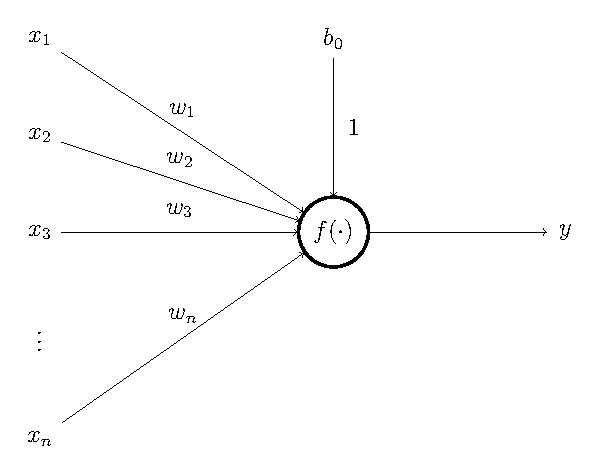
\includegraphics[width=0.9\linewidth]{figures/neuron.eps}
		\caption{Neural Network Node}
		\label{fig:modelNeuron_a}
	\end{subfigure}
	\begin{subfigure}{0.5\linewidth}
		\centering
		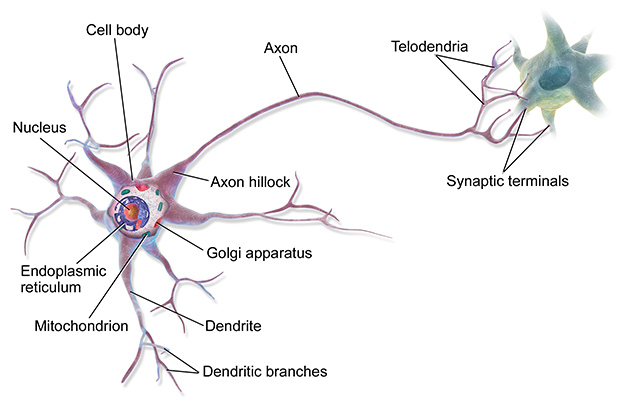
\includegraphics[width=0.9\linewidth]{figures/multipolarNeuron.png}
		\caption{Biological Neuron Diagram}
		\label{fig:modelNeuron_b}
	\end{subfigure}
		
	\caption{In Figure~\ref{fig:modelNeuron_a}. each input feature $x_i$ is weighted by its corresponding weight $w_i$. During the training procedure, these weights are adjusted so that the output $y$ approaches the target value. In Figure~\ref{fig:modelNeuron_b}, we see the diagram of an actual multi polar neuron. The dendrites, where the stimuli are received, plays a role similar to that of the input nodes. The axon transmits the signal to the synaptic terminals, that are similar to the $y$ output}
	\label{fig:modelNeuron}
\end{figure}


As far as the activation function is concerned, we can have several types. An immediate choice would be the \textbf{Binary Step Function} that  outputs -1 if the activation is \textbf{below} a given threshold and 1 otherwise. There can also be \textbf{real valued activation functions}, whose output is not binary, but rather that of a continuously differentiable function, such as the logistic sigmoid $\sigma(a) = \frac{1}{1 + \mathrm{e}^{-a}}$ or the hyperbolic tangent $\tanh(a)$. This aspect will prove useful for the usual training methods, that involve the computation of derivatives. In Figure~\ref{fig:activFunc} these activation functions are plotted.

\begin{figure}[H]
	\centering
	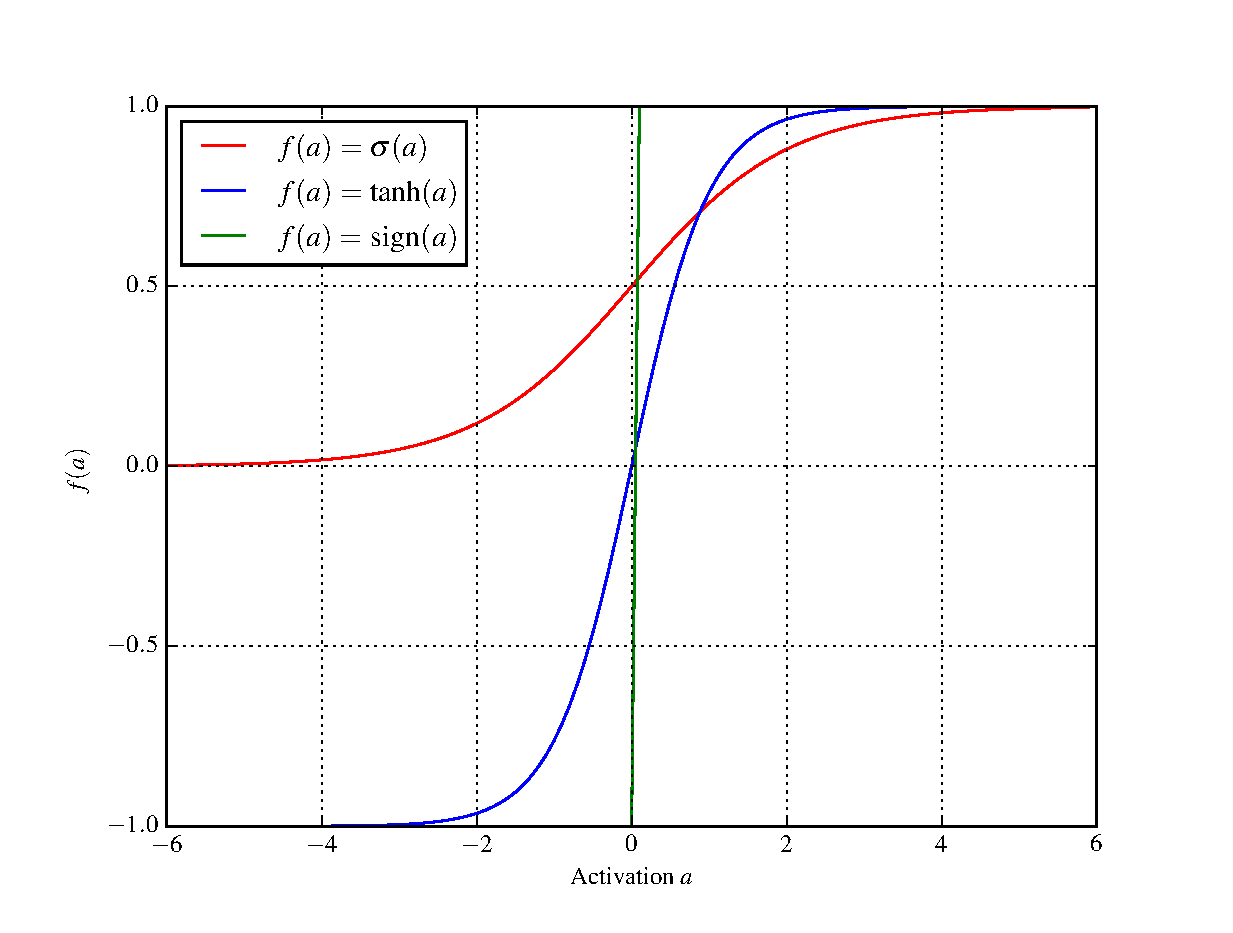
\includegraphics[width=0.9\linewidth]{figures/activFunc.eps}
	\caption{Three different activation functions. As you can see, the hyperbolic tangent has the same extreme value as the sign step function, but has a smooth transition between them, which can be interpreted as a \emph{soft decision} in the more ambiguous middle region, reflecting the degree of uncertainty on the decision. On the other hand, the sigmoid function goes from zero to one, and is also smooth like the hyperbolic tangent}.
	\label{fig:activFunc}
\end{figure}


A neuron by itself can be thought of as a simple linear regression, where we optimize the weight of each feature according to a target value, or function. While important in some applications, the main interest in ANN is to evaluate increasingly more complex models, and not a simple linear regression. This is achieved by \emph{chaining} nodes to one another, connecting the output of a given node to one of the inputs of another. We call \emph{layers} to a group of these nodes that occupy the same hierarchical position. There can be any number of layers, with any number of nodes, but most implementations generally have 3 layers: the \emph{initial} layer, the \emph{hidden} layer (in the middle) and the \emph{output} layer. Figure~\ref{fig:neuralnet} suggests a possible structure for a 3 layer ANN. 


\begin{figure}[H]
	\centering
	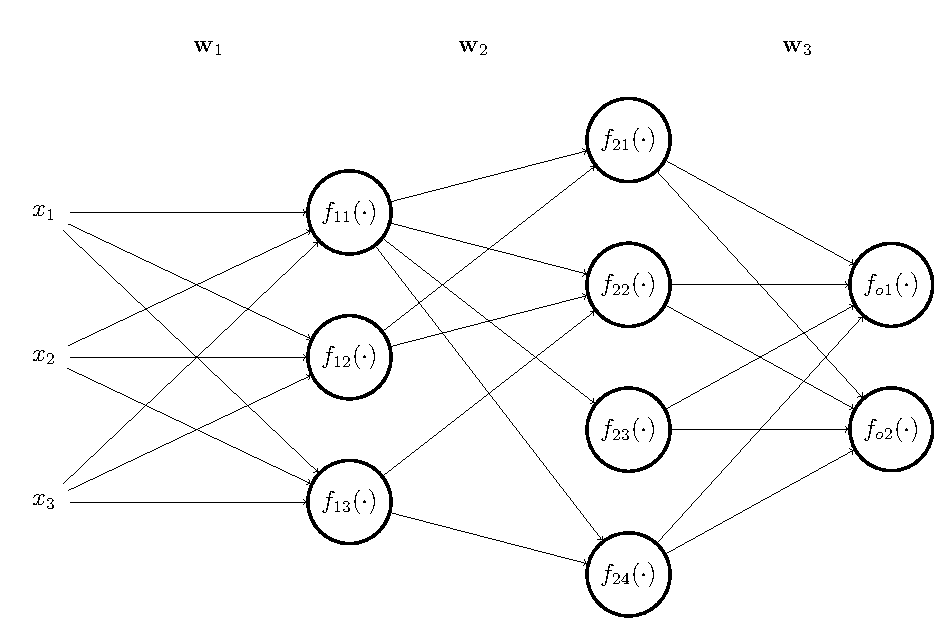
\includegraphics[width=0.9\linewidth]{figures/ann.eps}
	\caption{A three layer ANN. We have omitted some of the connections in the hidden layer, for simplification purposes. $\mb{w}_1$ represents the weight matrix of the input layer, $\mb{w}_2$ the weight matrix of the connections between the input layer and the hidden layer, and $\mb{w}_3$ the weight connections between the hidden and the output layer. $f_{ij}(\dots)$ is the activation function of the $j$-th neuron of the $i$-th layer. Since they can be different, I chose different indexes to each.}
	\label{fig:neuralnet}
\end{figure}

Regarding the training of ANNs, is is performed through a two-step process: first, a \textbf{feed-forward} step where the input is applied, and the activations are evaluated in succession up to the output neurons; then, the perform the \textbf{backpropagation} step, where we calculate the errors in each of the nodes, but now from the output to the input: the weights are updated and optimized using an iterative  method called \textit{Gradient Descent}, where if $\tau$ is the current time step, the next update on the weight matrix $\mb{w}^{(\tau+1)}$ is given by

\begin{equation}\label{eq:gradDesc}
	\mb{w}^{(\tau+1)} = \mb{w}^{(\tau)} - \eta \nabla E(\mb{w}^{(\tau)})
\end{equation}
where $E(\cdot)$ is the error function. As we can see, the weight matrix is moved in the direction that minimizes the error function the most, and $\eta$ controls how fast this is achieved, being the reason why it is called the \textbf{learning rate}.

The computation of gradient of the error function comprises the evaluation of its derivatives with respect to each weight of all network connections, $w_{ij}$. They are

\begin{equation}\label{eq:partialE}
	\frac{\partial E}{\partial w_{ji}} = \delta_j f(a_i)
\end{equation}
where $f(\cdot)$ is the activation function of the neuron and

\begin{equation}\label{eq:deltaj}
	\delta_j = f'(a_j) \sum_k w_{kj} \delta_k .
\end{equation}
The interpretation of these equations is simple. If $w_{ji}$ is the weight of the connection between the neuron $j$ we are considering and a neuron $i$ in a previous layer, then the sum over $k$ relates to all the neurons in the \emph{next} layer to which $j$ connects: this way, since the update on $w_{ji}$, according to~\ref{eq:gradDesc}, is given by

\begin{equation}\label{eq:update}
	w_{ji}^{(\tau+1)} = w_{ji}^{(\tau)} - \eta \frac{\partial E}{\partial w_{ji}}
\end{equation}
we see that, from~\ref{eq:partialE}  it simply is the product of the error of the current neuron, $\delta_j$, with the output of the previous neuron $f(a_i)$. In turn, from~\ref{eq:deltaj}, we see the recurrence relationship between it and the weighted sum of all posterior neurons that connect to it. Hence, the name backpropagation is now clear: we are, in fact, propagating the errors backwards into the neuron of interest, weighted by the corresponding weight, but now \emph{backwards} instead of forward, as before. For the output units, the $\delta_j$ is simply the difference between the produced output and the corresponding label for that sample. This two-step process is performed for every data point in out dataset. %%Place where I can include an algorithmic overview?
For a complete proof of the above formulas, see~\cite[chap. 5.3.1]{Bishop2006}.

\section{Recurrent Neural Networks}\label{sec:theorBack_rnn}
A Recurrent Neural Network (RNN) is, essentially, a regular ANN where some neurons (especially in the hidden layer) have \emph{feedback connections} to themselves, i.e. their outputs are fed as inputs. The relevance of this different structure is the possibility to retain \emph{sequence} information about the data. Before, each incoming data point only contributed to the training of the network, but no information about the correlation between themselves and the data points that preceded them did not influence the training step. They were regarded as if no temporal relationship existed, and therefore each data point is conditionally independent of any other. This is obviously not necessarily truth, and in fact there are many cases, where the correlation between data points is high for those closely spaced in time, in which it is actually completely false, as in video signals, audio signals, or other kinds of \emph{temporal sequences} of data. Therefore, the feedback connection of the neuron to himself acts as a kind of \emph{memory element} that takes into account in the present decision, the history of decisions previously taken, and hence the previous data. 
Figure~\ref{fig:recneuron} suggests a possible structure for a neuron of a hidden layer in an RNN, and also an alternate representation, where the structure is unfold through time.

%% METE AQUI A FIGURA

The training of an RNN is usually performed using a variation of Backpropagation, called \textbf{Backpropagation Through Time} (BPTT), that as the name implies, performs the same backpropagation procedure discussed for the ANNs, but now taking into account the unfolding of the network through a fixed training epoch $T$ like Figure~\ref{fig:recneuron}. Due to this very fact, this training procedure is memory and performance consuming, and so it will not be used in my final work, but instead a novel approach, the \textbf{Simulatneous Perturbation Stochastic Approximation}. 

Even though RNNs outperform static ANNs in sequence recognition problems~\cite{Bengio1991}, they fail to retain long-term dependencies. Of course that the weight training process is itself a form of memory, but the problem is that the weight update is much slower than the activations~\cite{Yoshua01}, and therefore this memory only retains short-term dependencies. This is because of the so-called \textbf{Vanishing Gradients Problem}~\cite{Yoshua94,Yoshua01}, where the error decays exponentially through time, and the impact of previous incoming data points on the training of the weights, and thus the current decision, quickly decreases. 


\section{Long Short-Term Memory Networks}\label{sec:theorBack_lstm}
To overcome the issue of failing to remember long-term dependencies, Hochreiter and Schmidhüber proposed, in 1997, a novel approach to the RNNs called the \textit{Long-Short Term Network}~\cite{Hoch97}. This section explains the main idea of this approach~\ref{sec:struct_lstm}, and also how it is trained\ref{sec:training_lstm}, serving as a support basis for the work of this thesis.
Although originally formulated in 1997, its formulation has been incrementally updated in~\cite{Gers00} and~\cite{Gers2000}, and the most current version is the one in~\cite{Graves05}. One of the inital proposers of LSTM, Prof. Jürgen Schmidhüber, did a survey on the most common variations of the structure~\cite{Greff15} last year, and this will the basis of this short theoretical presenation, as well as the work that will be developed in this thesis. 

\subsection{Structure, Operation and Equations}\label{sec:struct_lstm}
A single LSTM neuron is presented in Figure~\ref{fig:lstmneuron}. As we can see from the picture, we still have the recurrent connections from the regular RNNs, but now there are multiple entry points that control the flow of information through the network. Although ommited from the  picture, all the gates are biased, as is suggested in Equations~\ref{eq:equationsLstm}. The main components, their role and relevance, are explained as follows

\begin{itemize}

    \item \textbf{Input Gate} -- this is the input gate, where the importance of each feature of the input vector at time $t$, $\mb{x}^t$, and the output vector at the previous time step $\mb{y}^{t-1}$ is weighed in, producing an output $\mb{i}^{t}$.

    \item \textbf{Block Input Gate} -- as the name implies, this gate controls the flow of information from the input gate to the memory cell. It also receives the input vector and the previous output vector as inputs, but it does not have peephole connections and its dynamics are controlled by a different set of weights. The \textbf{activation function of this gate can be any}, but the most common choice is the \textbf{Hyperbolic Tangent}.

    \item \textbf{Forget Gate} -- its role is to control the contents of the Memory Cell, either to set them or reset them, using the \textit{Hadamard Elementwise} matrix multiplication of its output at time $t$, $\mb{c}^{(t)}$, with the contents of the memory unit at the previous time step, $\mb{c}^{(t-1)}$. The activation function of this gate is \textbf{always sigmoid}.

    \item \textbf{Output Block Gate} -- this gate has a role very similar to that of the Block Input Gate, but now it controls the information flow \textit{out} of the LSTM neuron, namely the activated Memory Cell output.

    \item \textbf{Memory Cell} -- the cornerstone of the LSTM neuron. This is the memory element of the neuron, where the previous state is kept, and updated accordingly to the dynamics of the gates that connect to it. Also, this is where the peephole connections come from:  

    \item \textbf{Output Activation} -- the output of the Memory Cell goes through this activation function that, as the gate activation function, can be any, but the \textit{hyperbolic tangent} is the most common choice.

    \item \textbf{Peepholes} -- direct connections \textit{from} the memory cell that allow for gates to `peep' the states of the memory cell. They were added after the initial 1997 formulation, and their absence was proven to have a minimal performance impact~\cite{Greff15}.
\end{itemize}

After this small conceptual definitions, that allow us to grasp some intuition on the operation of a \textit{single} LSTM cell, I can present the overview of a \textit{layer} of LSTM neurons and their formal mathematical formulation, that will be needed both for the high-level model and the HDL description. The operation of each gate of the layer is given by the following set of equations

\begin{align}
    \mb{z}^{(t)} & = g(\mb{W}_z \mb{x}^{(t)} + \mb{R}_z \mb{y}^{(t-1)} + \mb{b}_z) \\
    \mb{i}^{(t)} & = \sigma(\mb{W}_i \mb{x}^{(t)} + \mb{R}_i \mb{y}^{(t-1)} + \mb{p}_i \odot \mb{c}^{(t-1)} + \mb{b}_i) \\
    \mb{f}^{(t)} & = \sigma(\mb{W}_f \mb{x}^{(t)} + \mb{R}_f \mb{y}^{(t-1)} + \mb{p}_f \odot \mb{c}^{(t-1)} + \mb{b}_f) \\
    \mb{c}^{(t)} & = \mb{i}^{(t)} \odot \mb{z}^{(t)} + \mb{f}^{(t)} \odot \mb{c}^{(t-1)} \\
    \mb{o}^{(t)} & = \sigma(\mb{W}_o \mb{x}^{(t)} + \mb{R}_o \mb{y}^{(t-1)} + \mb{p}_o \odot \mb{c}^{(t)} + \mb{b}_o) \\
    \mb{c}^{(t)} & = \mb{o}^{(t)} \odot h(\mb{z}^{(t)}) 
\end{align}
The $i$-th element of the previous vectors in bold corresponds to the value of the gate of the $i$-th neuron of the layer, which is a very convenient and compact representation of the whole layer. Although useful for a high-level description in a programming language, the matrix representation  may not be suitable for a direct HDL port. In that case, all the above equations still hold, but instead of \textit{vectors} of outputs, we will have a single output, and we only use the appropriate value in the weight matrices $\mb{W}_{\cdot}$ and $\mb{R}_{\cdot}$
\begin{figure}
	\centering
	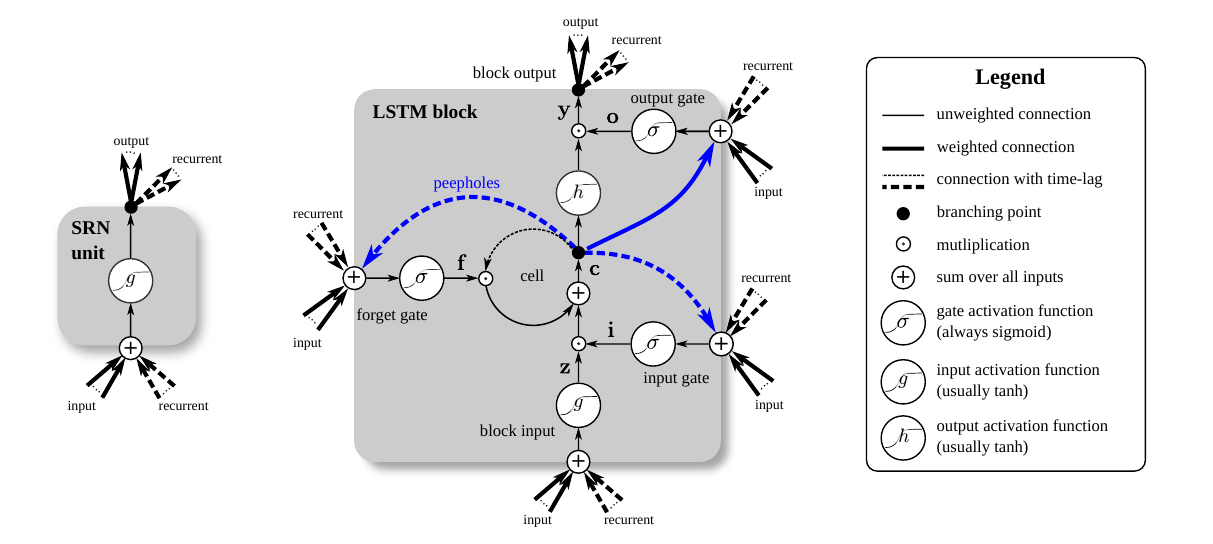
\includegraphics[width=0.9\linewidth]{figures/lstmneuron.png}
    \caption{A complete LSTM neuron, with all the features as described in~\cite{Graves05}}
	\label{fig:lstmneuron}
\end{figure}

\subsection{Training -- SPSA}\label{sec:training_lstm}
Since this work aims to perform on-chip learning, it is important to find a suitable learning scheme. Since I am aiming at an hardware implementation, and although the memory resources of nowadays FPGAs are abundant, one must find an algorithm that uses the less memory as possible (at the smallest performance cost possible), in order to use the additional memory, for instance, to add additional LSTM cells that can improve the performance of our system. 
That being said, we see that the usual training algorithms for LSTM cells -- i.e. Real-Time Recurrent Learning (RTRL), Truncated Backpropagation Through Time (BPTT) or a mixture of both~\cite{Graves05}~\cite{Hoch97}~\cite{Greff15} -- usually involve the storage of the deltas of each layer for every time instant in the training epoch (from $0$ to $T$), which is a highly non-scalable solution both in terms of memory and performance. A most efficient approach to training times series dependant structures like LSTM is the use of \textbf{Simultaneous Perturbation Stochastic Approximation} (SPSA)~\cite{Spall98}. The weight update for the $i$-th weight at the time step $t$ is given by 

\begin{equation}\label{eq:spsa_weightUpdate}
    \Delta w_i^{(t)} = \frac{J(\mb{w}^{(t)} + \beta \mb{s}^{(t)}) - J(\mb{w}^{(t)})}{\beta s_i^{(t)}}
\end{equation}
where $\beta$ is the magnitude of the perturbation to be introduced, $\mb{s}^{(t)}$ is a \textit{sign vector} whose $i$-th element, $s_i^{(t)}$, is either $-1$ or $1$. This way, we see that every weight is \textbf{randomly} incremented either by $-\beta$ or $\beta$, and we only need to keep a duplicate of the weight matrix with the perturbations, and we only need to evaluate the cost function twice per incoming sample. As for the \textit{update rule} is concerned, we have 

\begin{equation}\label{eq:spsa_updateRule}
    w_i^{(t+1)} = w_i^{(t)} - \eta \Delta w_i^{(t)}
\end{equation}
where $\eta$ is the learning rate, and $\Delta w_i^{(t)}$ is the update for the $i$-th weight evaluated in~\ref{eq:spsa_weightUpdate}.
According to the analysis performed in~\cite{Maeda05}, performing a second-order Taylor expansion at $\mb{w} = \mb{w}^{(t)}$, and taking the expected value of the equation, we get that

\begin{equation}\label{eq:spsa_gradProof}
    E(\Delta w_i^{(t)}) = \frac{\partial J(\mb{w}^{(t)})}{\partial w_i^{(t)}}
\end{equation}
that is, the weight update approximates the gradient of the cost function relative to that weight, and so the learning rule is a special form of \textit{Stochastic Gradient Descent}.

One last comment to be made concerning the update rule, is the hipothetical need for \textbf{limits} to the weight values, when the update rule exceeds $|w_{\text{max}}|$ (in that case, we set $w_i^{(t+1)} = \pm w_{\text{max}}$), which sometimes might be needed if the behaviour of the weight update is not appropriate~\cite{Maeda05}.





%% comment next 2 commands if numbered appendices are not used
\appendix
\chapter{Loren Ipsum} \label{ap1:loren}

Depois das conclusões e antes das referências bibliográficas,
apresenta-se neste anexo numerado o texto usado para preencher a
dissertação.

\section{O que é o \emph{Loren Ipsum}?}


\section{De onde Vem o Loren?}


%%----------------------------------------
%% Final materials
%%----------------------------------------

%% Bibliography
%% Comment the next command if BibTeX file not used
%% bibliography is in ``myrefs.bib''
\PrintBib{bibliography}
\bibliographystyle{IEEETran}
\bibliography{bibliography}
%% Index
%% Uncomment next command if index is required
%% don't forget to run ``makeindex thesis'' command
%\PrintIndex

\end{document}
